\documentclass{article}
\usepackage[]{graphicx}
\usepackage[]{color}
%% maxwidth is the original width if it is less than linewidth
%% otherwise use linewidth (to make sure the graphics do not exceed the margin)
\makeatletter
\def\maxwidth{ %
  \ifdim\Gin@nat@width>\linewidth
    \linewidth
  \else
    \Gin@nat@width
  \fi
}
\makeatother

\title{The Analysis of Data from Countries with HRT Reduction and Decrease in Breast Cancer}

\definecolor{fgcolor}{rgb}{0.345, 0.345, 0.345}
\newcommand{\hlnum}[1]{\textcolor[rgb]{0.686,0.059,0.569}{#1}}%
\newcommand{\hlstr}[1]{\textcolor[rgb]{0.192,0.494,0.8}{#1}}%
\newcommand{\hlcom}[1]{\textcolor[rgb]{0.678,0.584,0.686}{\textit{#1}}}%
\newcommand{\hlopt}[1]{\textcolor[rgb]{0,0,0}{#1}}%
\newcommand{\hlstd}[1]{\textcolor[rgb]{0.345,0.345,0.345}{#1}}%
\newcommand{\hlkwa}[1]{\textcolor[rgb]{0.161,0.373,0.58}{\textbf{#1}}}%
\newcommand{\hlkwb}[1]{\textcolor[rgb]{0.69,0.353,0.396}{#1}}%
\newcommand{\hlkwc}[1]{\textcolor[rgb]{0.333,0.667,0.333}{#1}}%
\newcommand{\hlkwd}[1]{\textcolor[rgb]{0.737,0.353,0.396}{\textbf{#1}}}%

\usepackage{framed}
\makeatletter
\newenvironment{kframe}{%
 \def\at@end@of@kframe{}%
 \ifinner\ifhmode%
  \def\at@end@of@kframe{\end{minipage}}%
  \begin{minipage}{\columnwidth}%
 \fi\fi%
 \def\FrameCommand##1{\hskip\@totalleftmargin \hskip-\fboxsep
 \colorbox{shadecolor}{##1}\hskip-\fboxsep
     % There is no \\@totalrightmargin, so:
     \hskip-\linewidth \hskip-\@totalleftmargin \hskip\columnwidth}%
 \MakeFramed {\advance\hsize-\width
   \@totalleftmargin\z@ \linewidth\hsize
   \@setminipage}}%
 {\par\unskip\endMakeFramed%
 \at@end@of@kframe}
\makeatother

\definecolor{shadecolor}{rgb}{.97, .97, .97}
\definecolor{messagecolor}{rgb}{0, 0, 0}
\definecolor{warningcolor}{rgb}{1, 0, 1}
\definecolor{errorcolor}{rgb}{1, 0, 0}
\newenvironment{knitrout}{}{} % an empty environment to be redefined in TeX

\usepackage{alltt}
\IfFileExists{upquote.sty}{\usepackage{upquote}}{}
\begin{document}

\maketitle

\section*{Introduction}

This set of analyses contains the R codes for the breast cancer study. The data were combined with the tables containing HRT usage data and the cancer incidence data were abstracted from the IARC ddatabases corresponding to the decline in the incidence rates three years after the reduction in the usage of HRT in the countries. In the following set of analyses, we present both the R codes that were used to generate the plots and analyses and the graphs and tables. 

\section*{ The Plot of Decrease in Breast Cancer with HRT Usage Reduction}

Figure 1 shows the plot of decrease in Ca incidence in the different countries (y axis ) and decrease in the use of HRT in the corresponding countries as well. 

\section*{The R Code to Produce the Plot}

\begin{knitrout}
\definecolor{shadecolor}{rgb}{0.969, 0.969, 0.969}\color{fgcolor}\begin{kframe}
\begin{alltt}
 \hlkwd{plot}\hlstd{(mydata}\hlopt{$}\hlstd{declinehrtuse, mydata}\hlopt{$}\hlstd{cadecrease,}
     \hlkwc{main} \hlstd{=} \hlstr{"Decrease in Breast Cancer Incidence with HRT"}\hlstd{,}
     \hlkwc{ylab} \hlstd{=} \hlstr{"Decrease in Breast Ca Incidence"}\hlstd{,}
     \hlkwc{xlab} \hlstd{=} \hlstr{"decrease in HRT usage"}\hlstd{)}

 \hlkwd{abline}\hlstd{(hrtuseca} \hlkwb{<-} \hlkwd{lm}\hlstd{(cadecrease} \hlopt{~} \hlstd{declinehrtuse,}
                   \hlkwc{data} \hlstd{= mydata))}
\end{alltt}
\end{kframe}
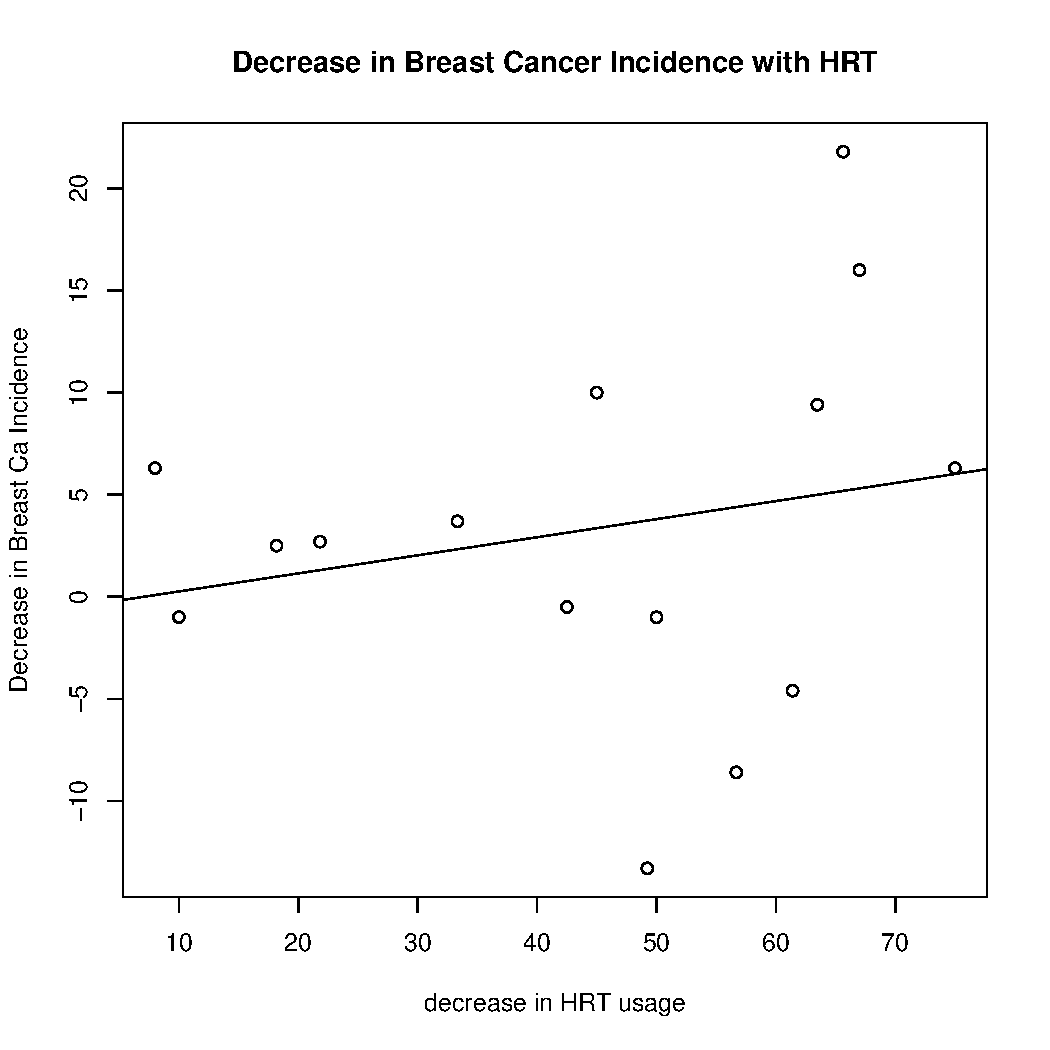
\includegraphics[width=\maxwidth]{figure/plotuseca-1} 
\begin{kframe}\begin{alltt}
 \hlcom{## let's take a look at the simple linear regression model,}

 \hlkwd{library}\hlstd{(knitr)}
\hlkwd{kable}\hlstd{(}\hlkwd{summary}\hlstd{(hrtuseca)}\hlopt{$}\hlstd{coef,} \hlkwc{digits}\hlstd{=}\hlnum{2}\hlstd{)}
\end{alltt}
\end{kframe}
\begin{tabular}{l|r|r|r|r}
\hline
  & Estimate & Std. Error & t value & p-value\\
\hline
(Intercept) & -0.62 & 5.53 & -0.11 & 0.91\\
\hline
Decline in HRT use & 0.09 & 0.11 & 0.79 & 0.45\\
\hline
\end{tabular}


\end{knitrout}
 
\section*{}

As can be seen in the above scatterplot, in general, with decrease in HRT usage, there was a corresponding reduction in Breast Cancer incidence three years after the reduction in HRT usage. However, this effect was not uniform as In six countries, there were also an increase in Breast Cancer incidence following reduction in HRT usage. 

In general, the fit line of the scatter plot indicate that with increase in decrease in HRT usage there was corresponding increase in reduction in Breast Cancer incidence as well. However it also suggests that the relationship between reduction in HRT usage and the corresponding reduction in Breast Cancer incidence followed a pattern, that the reduction in Breast Cancer was higher in those countries where the decrease in HRT usage was also very high, and this did not follow an exactly linear trend. A quadratic trend was explored by developing a quadratic model using a squared term of the HRT Reduction (that is, HRT Reduction Squared and putting this into the regression equation). The resulting summary of the coefficients of regression are shown as follows.

\section*{Table 2: Association between HRT Usage Reduction and Reduction in Br Ca incidence three years later -- quadratic model}

\begin{tabular}{l|r|r|r|r}
\hline
  & Estimate & Std. Error & t value & p-value\\
\hline
Intercept & 9.35 & 8.76 & 1.07 & 0.31\\
\hline
Decline in HRT use & -0.61 & 0.50 & -1.22 & 0.25\\
\hline
Decline in HRT Use Squared & 0.01 & 0.01 & 1.43 & 0.18\\
\hline
\end{tabular}

\section*{Removal of Data Points with Zero or Increased Incidence and Examination}

Next, information of the countries that had registered an increase in Breast Cancer three years following the reduction in HRT usage drop were removed from the data frame of analyses and information from only those countries were retained that had registered a drop in Breast Cancer incidence three years after drop in HRT usage. Figure 2 shows the relationship between the drop in HRT usage and the corresponding drop in Breast Cancer incidence three years after the HRT usage drop. 

\section*{The Code to remove the countries with zero or increase in Breast Cancer Incidence}

\begin{knitrout}
\definecolor{shadecolor}{rgb}{0.969, 0.969, 0.969}\color{fgcolor}\begin{kframe}
\begin{alltt}
 \hlstd{mydata2} \hlkwb{<-} \hlkwd{subset}\hlstd{(mydata, cadecrease} \hlopt{>=} \hlnum{0}\hlstd{)}

\hlcom{# print(summarize(mydata2))}

\hlkwd{plot}\hlstd{(mydata2}\hlopt{$}\hlstd{declinehrtuse, mydata2}\hlopt{$}\hlstd{cadecrease,}
         \hlkwc{main} \hlstd{=} \hlstr{"Decrease in Breast Cancer Incidence with HRT"}\hlstd{,}
         \hlkwc{ylab} \hlstd{=} \hlstr{"Decrease in Breast Ca Incidence"}\hlstd{,}
         \hlkwc{xlab} \hlstd{=} \hlstr{"decrease in HRT usage"}\hlstd{)}
  \hlkwd{abline}\hlstd{(hrtca2} \hlkwb{<-} \hlkwd{lm}\hlstd{(cadecrease} \hlopt{~} \hlstd{declinehrtuse,} \hlkwc{data} \hlstd{= mydata2))}
\end{alltt}
\end{kframe}

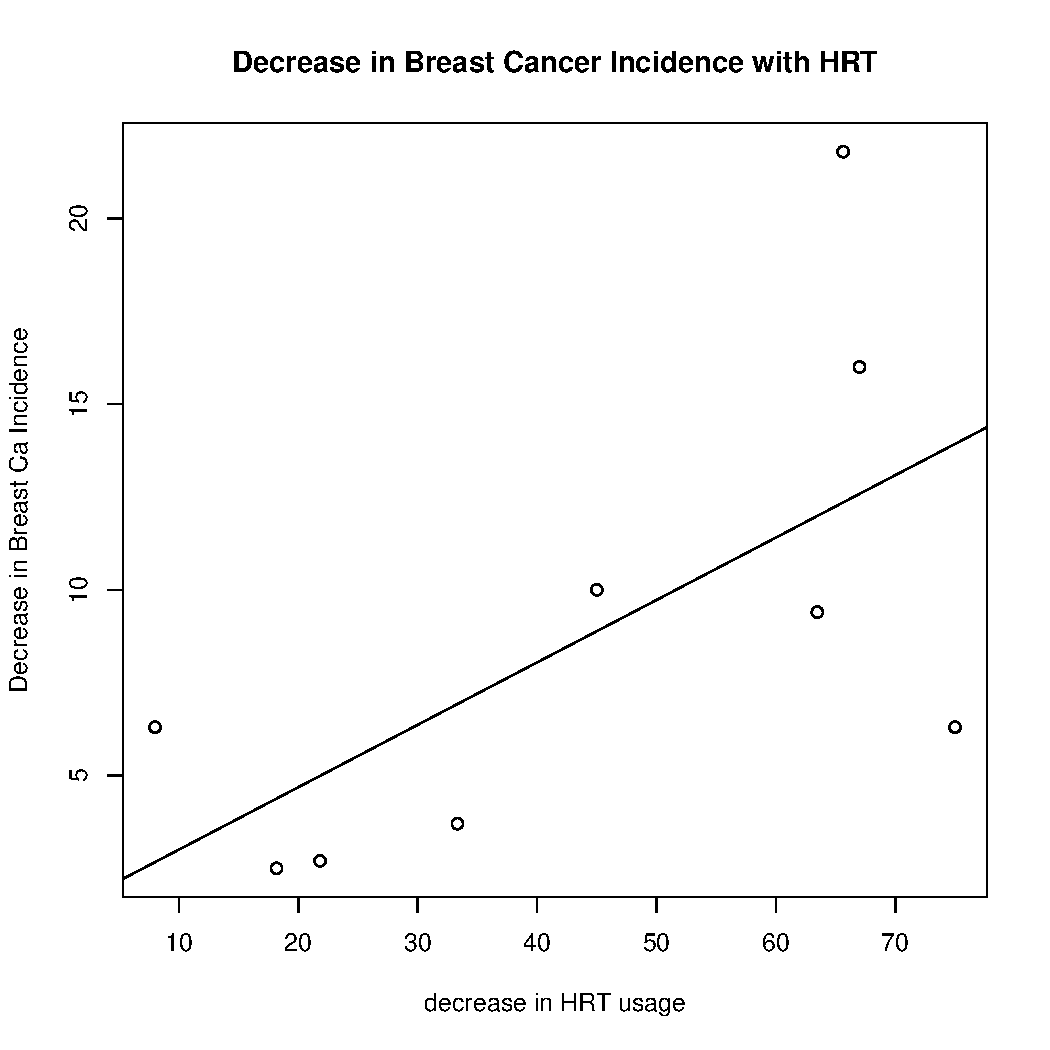
\includegraphics[width=\maxwidth]{figure/subsetting-1} 
\begin{kframe}\begin{alltt}
\hlkwd{kable}\hlstd{(}\hlkwd{summary}\hlstd{(hrtca2)}\hlopt{$}\hlstd{coef,} \hlkwc{digits} \hlstd{=} \hlnum{2}\hlstd{)}
\end{alltt}
\end{kframe}
\begin{tabular}{l|r|r|r|r}
\hline
  & Estimate & Std. Error & t value & p-value\\
\hline
(Intercept) & 1.32 & 3.81 & 0.35 & 0.74\\
\hline
Decline in HRT use & 0.17 & 0.08 & 2.21 & 0.06\\
\hline
\end{tabular}


\end{knitrout}

\section*{}

A very similar pattern of association can be observed between reduction in HRT usage and decrease in Breast Ca incidence, that is, as HRT usage has reduced in these countries, a corresponding decrease in Breast Cancer can be observed. Further, with higher levels of decreases in HRT usage the corresponding drop in Breast Cancer have been higher. 

\section*{Further Exploration with Categorisiing the Breast Cancer Incidence Drop and HRT Usage}

This was further examined in a subset analysis where the decrease in breast cancer incidence is divided into three equal groups: 

\begin{enumerate}
\item No to mild decrease in Breast Ca incidence (0-3.2)
\item Moderate decrease in Breast Ca incidence (3.2-8.6)
\item Large decrease in Breast Ca incidence (> 8.6)

\end{enumerate}


We examine graphically the reduction in HRT usage in the three groups of countries. 

\section*{The Code and the Plot for Reduction in HRT Usage in Y axis and Breast Ca incidence reduction in X axis}

\begin{knitrout}
\definecolor{shadecolor}{rgb}{0.969, 0.969, 0.969}\color{fgcolor}\begin{kframe}
\begin{alltt}
\hlkwd{barplot}\hlstd{(hrtcadeclevel,}
        \hlkwc{col} \hlstd{=} \hlstr{"black"}\hlstd{,} \hlkwc{main} \hlstd{=} \hlstr{"Bar Plot of % HRT Reduction"}\hlstd{,}
       \hlkwc{xlab} \hlstd{=} \hlstr{"Extent of Decrease in Breast Cancer"}\hlstd{,}
        \hlkwc{ylab} \hlstd{=} \hlstr{"Extent of Decrease in HRT Usage"}\hlstd{,}

       \hlkwc{ylim} \hlstd{=} \hlkwd{c}\hlstd{(}\hlnum{0}\hlstd{,} \hlnum{70}\hlstd{))}
\end{alltt}
\end{kframe}
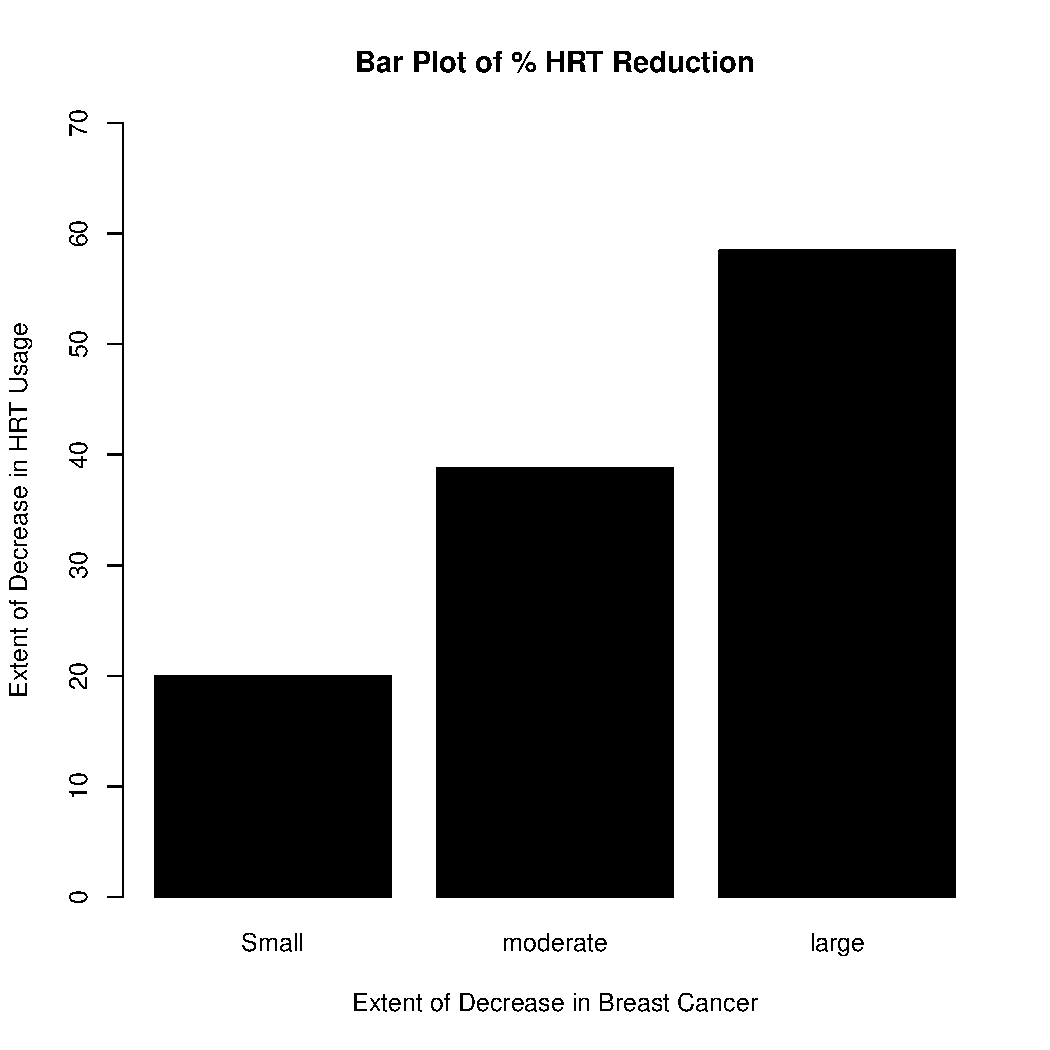
\includegraphics[width=\maxwidth]{figure/barplot1-1} 

\end{knitrout}

\section*{Graphical Exploration of Reduction in HRT Usage in X axis (categorised) and reduction in Incidence of Breast Cancer three years after the last registered year of HRT usage drop}

This was further explored with drawing bar plots where the reduction in Breast Ca incicence three years after the last known year for drop in HRT usage was plotted against the extent to which the countries showed a drop in HRT usage. This is essentially the above plot turned on the other side. In addition, a series of box plots are also shown here that suggests that at higher level of reduction in HRT usage, the corresponding drop in the Breast Cancer incidence were high. The usage of reduction in HRT was classified as follows:

\begin{enumerate}
\item Lowest level of drop, 30\% or lower in the drop from peak
\item Middle Level of drop, between 30 to 65.5 \%
\item High level of drop in HRT usage, more than 65.5 \%
\end{enumerate}


\section*{The Code and the Plots are Shown Below} 

\begin{knitrout}
\definecolor{shadecolor}{rgb}{0.969, 0.969, 0.969}\color{fgcolor}\begin{kframe}
\begin{alltt}
\hlcom{## Now, analyse the the extent to reduction in HRT usage}
\hlcom{##print(summary(mydata2$declinehrtuse))}
\hlcom{## given the minimum 8, q1 21.8, q3 65.5, highest 75}
\hlstd{mydata2}\hlopt{$}\hlstd{hrtdeclinecat} \hlkwb{<-} \hlkwd{cut}\hlstd{(mydata2}\hlopt{$}\hlstd{declinehrtuse,}
                            \hlkwc{breaks} \hlstd{=} \hlkwd{c}\hlstd{(}\hlnum{8}\hlstd{,} \hlnum{30}\hlstd{,} \hlnum{65.6}\hlstd{,} \hlnum{75}\hlstd{))}
\hlkwd{levels}\hlstd{(mydata2}\hlopt{$}\hlstd{hrtdeclinecat)} \hlkwb{<-} \hlkwd{c}\hlstd{(}\hlstr{"lt 30"}\hlstd{,} \hlstr{"30-65.5"}\hlstd{,} \hlstr{"gt 65.5"}\hlstd{)}

\hlstd{cadeclevel} \hlkwb{<-} \hlkwd{tapply}\hlstd{(mydata2}\hlopt{$}\hlstd{cadecrease, mydata2}\hlopt{$}\hlstd{hrtdeclinecat, mean)}
\end{alltt}
\end{kframe}
\end{knitrout}

It can be seen that there is a progressive increase in the reduction in Breast Cancer incidence three years after the reduction in HRT usage  

This can be further examined using the boxplots of reduction
\begin{knitrout}
\definecolor{shadecolor}{rgb}{0.969, 0.969, 0.969}\color{fgcolor}\begin{kframe}
\begin{alltt}
\hlkwd{boxplot}\hlstd{(mydata2}\hlopt{$}\hlstd{cadecrease} \hlopt{~} \hlstd{mydata2}\hlopt{$}\hlstd{hrtdeclinecat)}
\end{alltt}
\end{kframe}
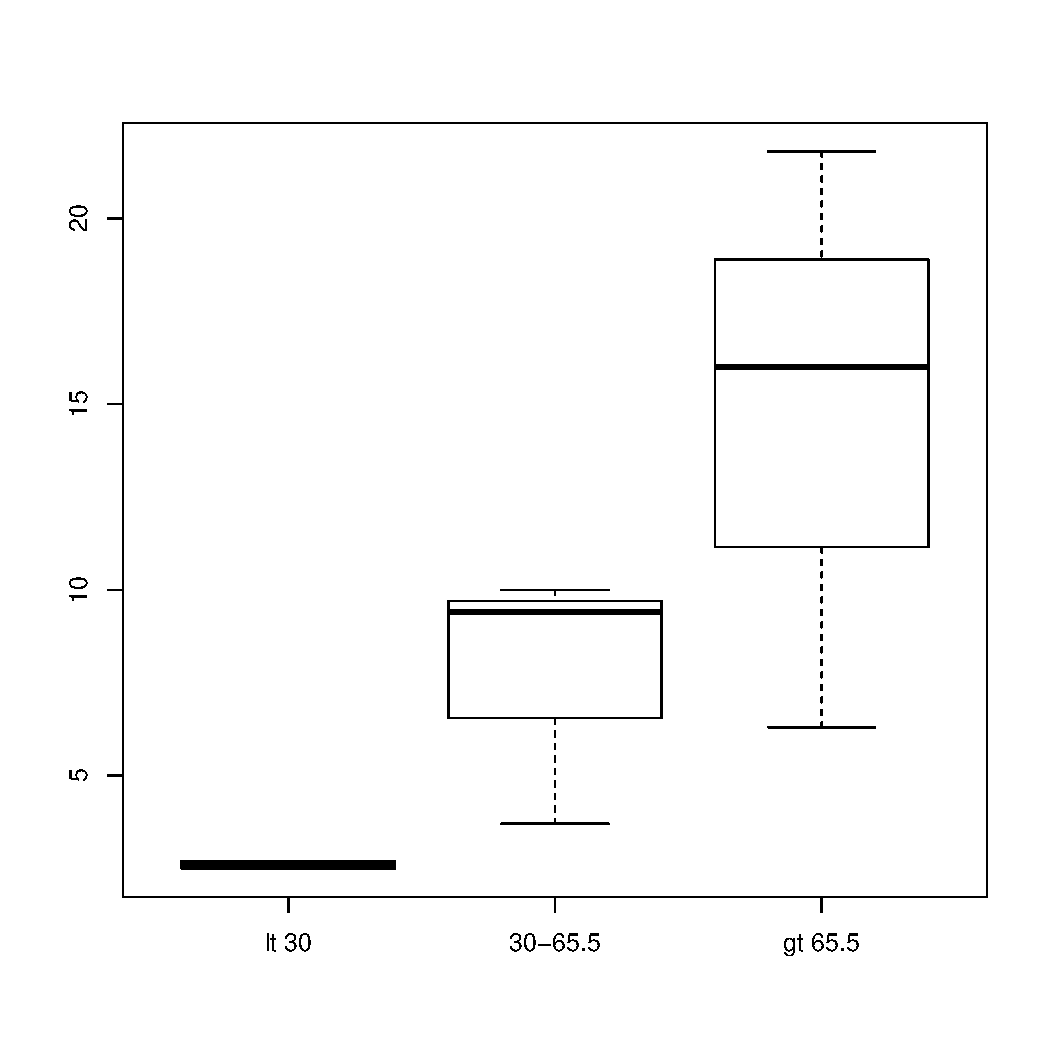
\includegraphics[width=\maxwidth]{figure/box-1} 

\end{knitrout}

Also as the barplot shows,
\begin{knitrout}
\definecolor{shadecolor}{rgb}{0.969, 0.969, 0.969}\color{fgcolor}\begin{kframe}
\begin{alltt}
\hlkwd{barplot}\hlstd{(cadeclevel,}
      \hlkwc{col} \hlstd{=} \hlstr{"black"}\hlstd{,} \hlkwc{main} \hlstd{=} \hlstr{"Bar Plot of Breast Ca Reduction"}\hlstd{,}
     \hlkwc{ylab} \hlstd{=} \hlstr{"Extent of Decrease in Breast Cancer"}\hlstd{,}
        \hlkwc{xlab} \hlstd{=} \hlstr{"Extent of Decrease in HRT Usage"}\hlstd{,}

       \hlkwc{ylim} \hlstd{=} \hlkwd{c}\hlstd{(}\hlnum{0}\hlstd{,} \hlnum{20}\hlstd{))}
\end{alltt}
\end{kframe}
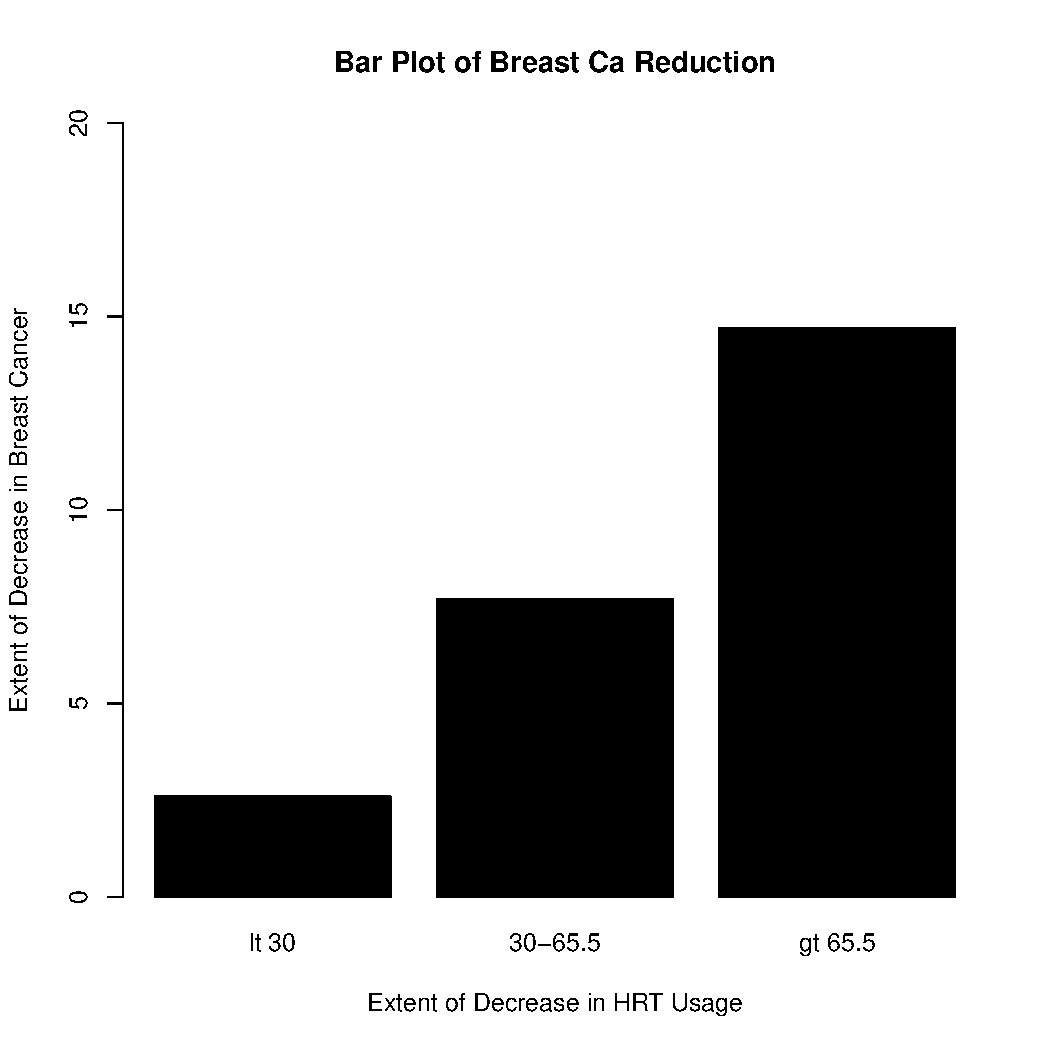
\includegraphics[width=\maxwidth]{figure/barplot2-1} 

\end{knitrout}

\end{document}
